\begin{abox}
	Practise Set-2
\end{abox}
\begin{enumerate}
	\item The graph of the function $f(x)=\left\{\begin{array}{ll}1 & \text { for } 2 n \leq x \leq 2 n+1 \\ 0 & \text { for } 2 n+1 \leq x \leq 2 n+2\end{array}\right.$ where $n=(0,1,2, \ldots \ldots)$ is shown below. Its Laplace transform $\tilde{f}(s)$ is
	{	\exyear{NET/JRF(DEC-2011)}}
	
	\begin{figure}[H]
		\centering
		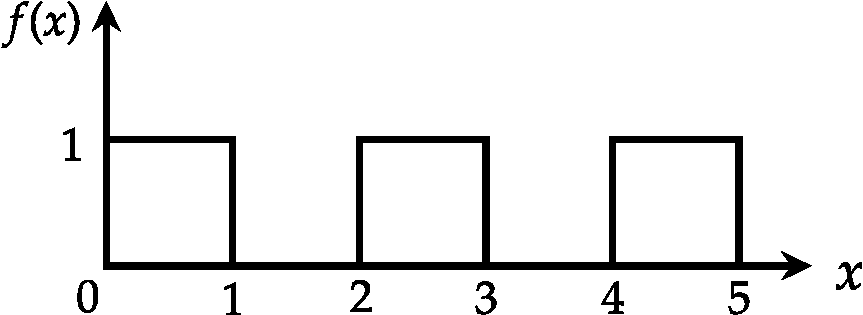
\includegraphics[height=2.7cm,width=7.5cm]{diagram-20211005(9)-crop}
	\end{figure}
	\begin{tasks}(4)
		\task[\textbf{A.}] $\frac{1+e^{-s}}{s}$
		\task[\textbf{B.}] $\frac{1-e^{-s}}{s}$
		\task[\textbf{C.}] $\frac{1}{s\left(1+e^{-s}\right)}$
		\task[\textbf{D.}]  $\frac{1}{s\left(1-e^{-s}\right)}$
	\end{tasks}
	\begin{answer}
		\begin{align*}
		L(f(x))&=\int_{0}^{\infty} e^{-s x} f(x) d x\\&=\int_{0}^{1} e^{-s x} \cdot 1 d x+\int_{1}^{2} e^{-s x} \cdot 0 d x+\int_{2}^{3} e^{-s x} \cdot 1 d x+\ldots \ldots\\
		&=\left[\frac{e^{-s x}}{-s}\right]_{0}^{1}+0+\left[\frac{e^{-s x}}{-s}\right]_{2}^{3}+\ldots \ldots\\&=\frac{1}{-s}\left[e^{-s}-1\right]+\frac{1}{-s}\left[e^{-3 s}-e^{-2 s}\right]+\ldots \ldots\\
		&=\frac{1}{-s}\left[-1+e^{-s}-e^{-2 s}+e^{-3 s}+\ldots \ldots . .\right]\\&=\frac{1}{s}\left[1-e^{-s}+e^{-2 s}-e^{-3 s}+\ldots .\right]\\
		\text{Since }S_{\infty}&=\frac{a}{1-r}\text{ where }r=-e^{-s}\text{ and }a\\&=1 \Rightarrow S_{\infty}=\frac{1}{s}\left[\frac{1}{\left(1+e^{-s}\right)}\right]
		\end{align*}
	\end{answer}
	\item The inverse Laplace transforms of $\frac{1}{s^{2}(s+1)}$ is
	{\exyear{NET/JRF(JUNE-2013)}}
	
	\begin{tasks}(4)
		\task[\textbf{A.}] $\frac{1}{2} t^{2} e^{-t}$
		\task[\textbf{B.}] $\frac{1}{2} t^{2}+1-e^{-t}$
		\task[\textbf{C.}] $t-1+e^{-t}$
		\task[\textbf{D.}] $\frac{1}{2} t^{2}\left(1-e^{-t}\right)$
	\end{tasks}
	\begin{answer}
		\begin{align*}
		f(s)&=\frac{1}{s+1} \Rightarrow f(t)=e^{-t} \Rightarrow L^{-1}\left[\frac{1}{s(s+1)}\right]\\&=\int_{0}^{t} e^{-t} d t=\left(-e^{-t}\right)_{0}^{t}=\left(-e^{-t}+1\right)\\
		\Rightarrow L^{-1}\left[\frac{1}{s^{2}(s+1)}\right]&=\int_{0}^{t}\left(-e^{-t}+1\right) d t\\&=\left(e^{-t}+t\right)_{0}^{t}=e^{-t}+t-1
		\end{align*}
		So the correct answer is \textbf{Option (C)}
	\end{answer}
	\item The Laplace transform of
	$$
	f(t)=\left\{\begin{array}{cc}
	\frac{t}{T}, & 0<t<T \\
	1 & t>T
	\end{array}\right.
	$$
	is
	{\exyear{NET/JRF(DEC-2016)}}
	
	\begin{tasks}(4)
		\task[\textbf{A.}] $\frac{-\left(1-e^{-s T}\right)}{s^{2} T}$
		\task[\textbf{B.}] $\frac{\left(1-e^{-s T}\right)}{s^{2} T}$
		\task[\textbf{C.}] $\frac{\left(1+e^{-s T}\right)}{s^{2} T}$
		\task[\textbf{D.}] $\frac{\left(1-e^{s T}\right)}{s^{2} T}$
	\end{tasks}
	\begin{answer}
		\begin{align*}
		\intertext{we can write}
		f(t)&=\left[u_{0}(t)-u_{T}(t)\right] \frac{t}{T}+u_{T}(t)\\&=\left[1-u_{T}(t)\right] \frac{t}{T}+u_{T}(t)=\frac{t}{T}-u_{T}(t) \frac{t}{T}+u_{T}(t)
		\intertext{Hence the transform of $f(t)$ is}
		L\{f(t)\}&=L\left\{\frac{t}{T}\right\}-L\left\{u_{T}(t)\left[\frac{(t-T)+T}{T}\right]\right\}+L\left\{u_{T}(t)\right\}\\
		&=\frac{1}{s^{2} T}-\frac{e^{-s T}}{T}\left(\frac{1}{s^{2}}+\frac{T}{s}\right)+\frac{e^{-s T}}{s}=\frac{1-e^{-s T}}{s^{2} T}
		\end{align*}
		So the correct answer is \textbf{Option (B)}
	\end{answer}
	\item Consider the differential equation $\frac{d y}{d t}+a y=e^{-b t}$ with the initial condition $y(0)=0$. Then the Laplace transform $Y(s)$ of the solution $y(t)$ is
	{\exyear{NET/JRF(DEC-2017)}}
	
	\begin{tasks}(4)
		\task[\textbf{A.}] $\frac{1}{(s+a)(s+b)}$
		\task[\textbf{B.}] $\frac{1}{b(s+a)}$
		\task[\textbf{C.}] $\frac{1}{a(s+b)}$
		\task[\textbf{D.}] $\frac{e^{-a}-e^{-b}}{b-a}$
	\end{tasks}
	\begin{answer}
		\begin{align*}
		\text{Given }\frac{d y}{d t}+a y&=e^{-b t}
		\intertext{Taking Laplace transform of both sides}
		\text{	We obtain}\\
		L\left\{\frac{d y}{d t}\right\}+a L\{y(t)\}&=L\left\{e^{-b t}\right\} \Rightarrow s Y(s)-y(0)+a Y(s)=\frac{1}{s+b}\\
		\text{Since, }	y(0)&=0,\text{ we obtain}\\
		(s+a) Y(s)&=\frac{1}{s+b} \Rightarrow Y(s)=\frac{1}{(s+a)(s+b)}
		\end{align*}
		So the correct answer is \textbf{Option (A)}
	\end{answer}
	\item If $f(x)=\left\{\begin{array}{ll}0 & \text { for } x<3, \\ x-3 & \text { for } x \geq 3\end{array}\right.$ then the Laplace transform of $f(x)$ is
	{\exyear{GATE 2010}}
	
	\begin{tasks}(4)
		\task[\textbf{A.}] $s^{-2} e^{3 s}$
		\task[\textbf{B.}] $s^{2} e^{3 s}$
		\task[\textbf{C.}] $s^{-2}$
		\task[\textbf{D.}] $s^{-2} e^{-3 s}$
	\end{tasks}
	\begin{answer}
		\begin{align*}
		L\{f(x)\}&=\int_{0}^{\infty} e^{-s x} f(x) d x\\&=\int_{0}^{3} e^{-s x} f(x) d x+\int_{3}^{\infty} e^{-s x} f(x) d x\\&=\int_{3}^{\infty}(x-3) e^{-s x} d x\\
		L\{f(x)\}&=\left.(x-3) \frac{e^{-s x}}{-s}\right|_{3} ^{\infty}-\int_{3}^{\infty} 1 \cdot\left(\frac{e^{-s x}}{-s}\right) d x\\&=0+\frac{1}{s} \int_{3}^{\infty} e^{-s x} d x\\&=\frac{1}{s}\left[\frac{e^{-s x}}{-s}\right]_{3}^{\infty}=s^{-2} e^{-3 s}
		\end{align*}
		So the correct answer is \textbf{Option (D)}
	\end{answer}
	\item The Laplace transform of $\frac{(\sin (a t)-a t \cos (a t))}{\left(2 a^{3}\right)}$ is 
	{\exyear{JEST 2018}}
	
	\begin{tasks}(4)
		\task[\textbf{A.}] $\frac{2 a s}{\left(s^{2}+a^{2}\right)^{2}}$
		\task[\textbf{B.}]$\frac{s^{2}-a^{2}}{\left(s^{2}+a^{2}\right)^{2}}$
		\task[\textbf{C.}]$\frac{1}{(s+a)^{2}}$
		\task[\textbf{D.}]$\frac{1}{\left(s^{2}+a^{2}\right)^{2}}$
	\end{tasks}
\end{enumerate}
\colorlet{ocre1}{ocre!70!}
\colorlet{ocrel}{ocre!30!}
\setlength\arrayrulewidth{1pt}
\begin{table}[H]
	\centering
	\arrayrulecolor{ocre}
	\begin{tabular}{|p{1.5cm}|p{1.5cm}||p{1.5cm}|p{1.5cm}|}
		\hline
		\multicolumn{4}{|c|}{\textbf{Answer key}}\\\hline\hline
		\rowcolor{ocrel}Q.No.&Answer&Q.No.&Answer\\\hline
		1&\textbf{C} &2&\textbf{C}\\\hline 
		3&\textbf{B} &4&\textbf{A} \\\hline
		5&\textbf{D} &6 &\textbf{D} \\\hline
		
		
	\end{tabular}
\end{table}